%	!Mode::"UTF-8"
%	本模板设置改自北京大学交叉学院 王宇哲学长和北京大学化学与分子工程学院 王应泽同学的分享,特此感谢!
%	模板制作:北京大学化学与分子工程学院 王梓涵
%	Email:2100011837@stu.pku.edu.cn
%	本模板仅适用于北京大学物理化学实验报告,其他学校请自行修改
%	吐槽:Latex用于写物化实验报告还是过于繁琐了,不过还是比Word好用多了(๑•̀ㅂ•́)و✧ (此吐槽由copilot自动生成,模板作者认为word更好用)
%	本模板仅供交流学习使用,不可用作商业用途。

\documentclass[12pt]{article}

%	页面设置
\usepackage{geometry}
\geometry{left=2.5cm, right=2.5cm, top=2.5cm, bottom=2.5cm}
\usepackage{graphicx}
\usepackage{ctex}
\usepackage{fontspec}
\usepackage{setspace}
\usepackage[usenames,dvipsnames]{xcolor}
\usepackage{titlesec}

%	字体设置
\setmainfont{Times New Roman}
\setCJKmainfont{SimSun}
\setCJKsansfont{SimHei}

%	表格设置\
\usepackage{array,colortbl}
\usepackage{makecell}
\newcommand{\addcell}[2][4]{\makecell{\zihao{#1}\textsf{#2}}}
\usepackage{titlesec}
\usepackage{booktabs}
\usepackage{ragged2e} 
\usepackage{multirow}
\usepackage{tabularx}

% 网址设置
\usepackage{hyperref}
\hypersetup{hidelinks,
	colorlinks=true,
	allcolors=black,
	pdfstartview=Fit,
	breaklinks=true}


%	设置图注、表注
\usepackage{caption}
\usepackage{bicaption}
\captionsetup{labelsep=quad, font={small, bf}, skip=2pt}
\DeclareCaptionOption{english}[]{
    \renewcommand\figurename{Fig.}
    \renewcommand\tablename{Table}
}
\captionsetup[bi-second]{english}

%	设置页眉
\usepackage{fancyhdr}
\usepackage{xpatch}
\pagestyle{fancy}
\fancypagestyle{preContent}{
    	\fancyhead[L]{\zihao{-5} 物理化学实验}
    	\fancyhead[C]{\zihao{-5} 实验五\ \ 蔗糖的转化}
    	\fancyhead[R]{\zihao{-5} 2100011837\ 王梓涵}
		\renewcommand{\headrulewidth}{2pt}
		\renewcommand{\footrulewidth}{1pt}
		\xpretocmd\headrule{\color{BrickRed}}{}{\PatchFailed} % 设置页眉分割线颜色
		\xpretocmd\footrule{\color{BrickRed}}{}{\PatchFailed} % 设置页脚分割线颜色
}
\pagestyle{preContent}



%	设置首页页眉及取消首页页脚 若不需要首页页眉 请注释掉下列内容
\fancypagestyle{plain}{
	\fancyhead[L]{\zihao{-5} 物理化学实验}
    \fancyhead[C]{\zihao{-5} 实验五\ \ 蔗糖的转化}
	\fancyhead[R]{\zihao{-5} 2100011837\ 王梓涵}
	\cfoot{}
}

%	设置标题格式
\titleformat*{\section}{\color{Mahogany}\zihao{4}\sffamily}
\titleformat*{\subsection}{\zihao{-4}\sffamily}
\titleformat*{\subsubsection}{\zihao{-4}\sffamily}
\titlespacing*{\section}{0pt}{10pt}{10pt}
\titlespacing*{\subsection}{0pt}{10pt}{5pt}
\titlespacing*{\subsubsection}{0pt}{10pt}{5pt}


%	设置引用格式(ACS格式规范)
%	注意:请安装JabRef
%	JabRef使用参考:https://blog.csdn.net/weixin_44191286/article/details/85698921
\usepackage[super,round,comma,compress]{natbib}

%	数学公式增强
\usepackage{amsmath}
\usepackage{amssymb}

%	单位与数学式
\usepackage{siunitx}

% 其他添加
\usepackage[version=4]{mhchem}

%	设置封面
\begin{document}
    % 标题页
    \begin{titlepage}
    	% 页眉
    	\thispagestyle{plain}
        % 校徽图片
        \begin{figure}[h]
            \centering
            \includegraphics{pku.png}
        \end{figure}
        \vspace{24pt}
        % 标题
        \centerline{\zihao{-0} \textsf{\textcolor{Mahogany}{物理化学实验报告}}}
        \vspace{40pt} % 空行
        \begin{center}
            \begin{tabular}{cp{14.1cm}}
                % 题目
                \addcell[2]{题目:} & \addcell[1]{蔗糖的转化} \\
                \cline{2-2}
            \end{tabular}
        \end{center}
        \vspace{20pt} % 空行
        \begin{center}
            \doublespacing
            \begin{tabular}{cp{5cm}}
                % 姓名
                \addcell{姓\phantom{空格}名:\ } & \addcell{王梓涵} \\
                \cline{2-2}
                % 学号
                \addcell{学\phantom{空格}号:\ } & \addcell{2100011837}\\
                \cline{2-2}
                % 组别
                \addcell{组\phantom{空格}别:\ } & \addcell{22组} \\
                \cline{2-2}
                % 实验日期
                \addcell{实验日期:\ } & \addcell{2023.10.26}\\
                \cline{2-2}
                % 室温
                \addcell{室\phantom{空格}温:\ } & \addcell{295.15\ K}\\
                \cline{2-2}
                % 大气压强
                \addcell{大气压强:\ } & \addcell{101.08\ kPa}\\
                \cline{2-2}
            \end{tabular}
            \begin{tabular*}{\textwidth}{c}
                \\ % 这是空行
                \\ % 这是空行
                \\ % 这是空行
                \hline % 分割线
            \end{tabular*}
        \end{center}
        % 摘要
        \textsf{\textcolor{BrickRed}{摘\ \ 要}}\ \  \  本实验利用目视旋光仪测定蔗糖转化过程中体系旋光度的变化,间接得到了蔗糖的浓度变化,从而计算蔗糖转化反应的化学反应动力学常数。实验中加入浓度为$3.13\ \ {\rm M}$、$4.12\ \ {\rm M}$和$6.16\ \ {\rm M}$的盐酸时,蔗糖转化反应的速率常数$k$分别为$7.82\times10^{-4}\ \ s^{-1}$、$1.26\times10^{-3}\ \ s^{-1}$和$3.17\times10^{-3}\ \ s^{-1}$。计算了对应的半衰期$t_{1/2}$分别为$885\ \ s$、$550\ \ s$和$220\ \ s$。实验结果验证了蔗糖转化反应的对于蔗糖为一级反应,对氢离子为二级反应。
        \\
        \\
        % 关键字
        \textsf{\textcolor{BrickRed}{关键词}}\ \ 蔗糖的转化;目视旋光仪;反应速率常数;旋光度;一级反应
    \end{titlepage}

    \section{引言}
		\subsection{实验目的}
			本实验的实验目的主要有以下几点\citealp{physchemlab}:\par
			\ \ \ \ \ \ \ \ 1. 了解一级反应动力学的动力学特征。\par
			\ \ \ \ \ \ \ \	2. 测定蔗糖转化的反应级数、速率常数和$t_{1/2}$\par
			\ \ \ \ \ \ \ \	3. 掌握旋光仪的原理及其使用方法。\par

		\par
			\subsection{实验原理和实验方法}
				实验原理和实验方法在实验预习报告中如\textbf{图1}所示: \par
		\begin{figure}[h]
			\centering
			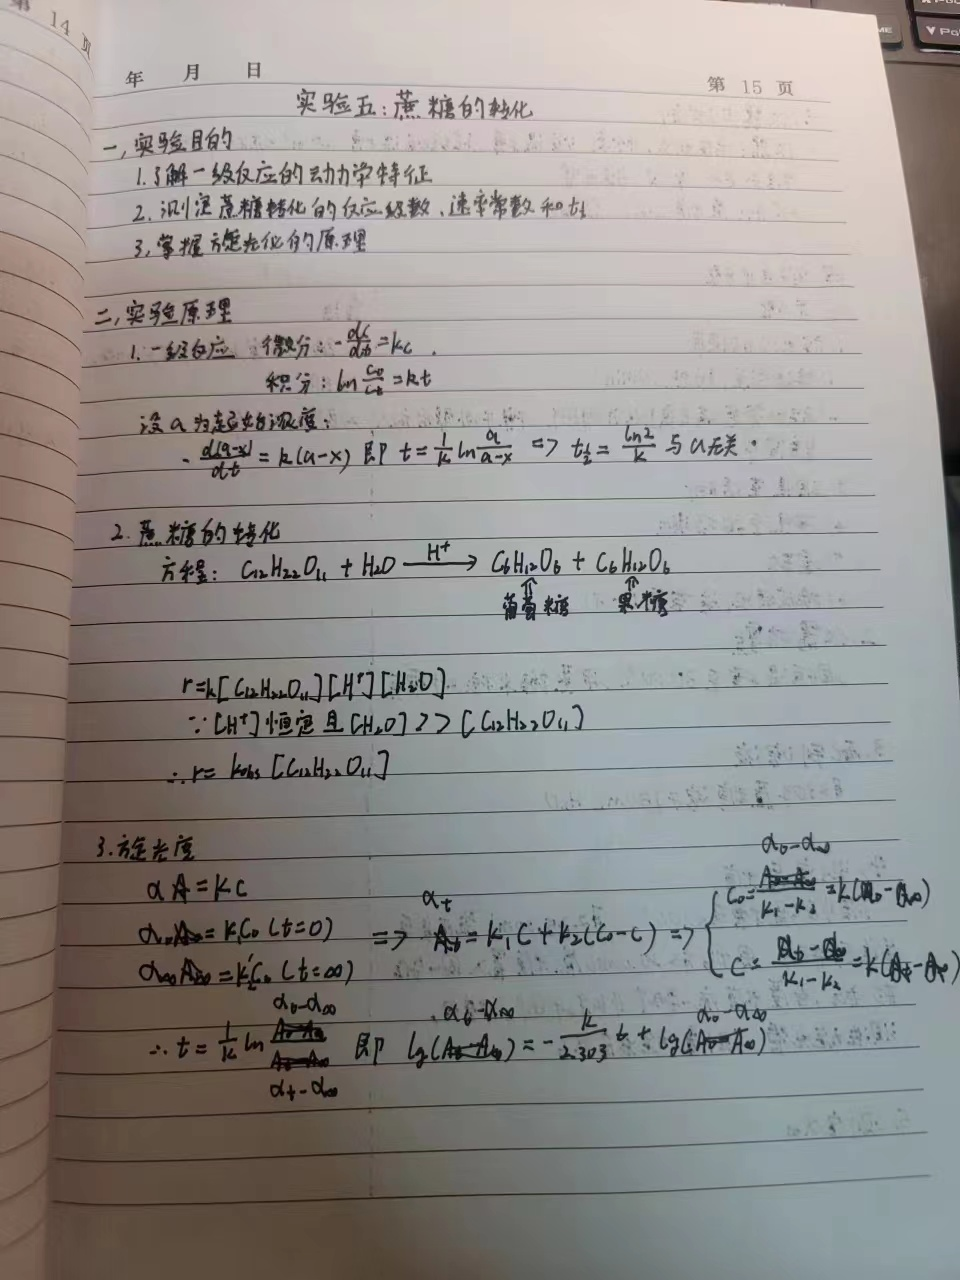
\includegraphics[width=0.67\textwidth]{1.png}
			\bicaption{实验预习报告的实验原理部分}{The principle part of the experiment in the experiment preview report}
		\end{figure}

	     
    \section{实验部分}

    	\subsection{仪器和试剂}
    		仪器:\ \  WXG-4目视旋光仪,超级恒温槽,$250\ \ {\rm mL}$烧杯,$25\ \ {\rm mL}$移液管,$100\ \ {\rm mL}$磨口锥形瓶,$100\ \ {\rm mL}$量筒,恒温旋光管。
			试剂:\ \  纯水,蔗糖(AR),$3$种不同浓度的盐酸(AR,浓度分别为$3.13\ \ {\rm M}$、$4.12\ \ {\rm M}$、$6.16\ \ {\rm M}$)。

    	 \subsection{实验内容\citealp{physchemlab}}
			\subsubsection{旋光仪零点校准}
			接通WXG-4目视旋光仪电源,打开电源开关预热$10\ \ {\rm min}$,待完全发出钠黄光。洗净恒温旋光管,连接好恒温水管路,将旋光管加满去离子水,并将管内气泡从加液口排净,旋光管外壁残液用滤纸擦净、两端玻璃片用擦镜纸擦净,放入旋光仪镜筒中。
			调节调焦螺旋,使视场中三分视场分界线最清晰。调节读盘转动手轮,至三分视场消失,视野暗度相同,从读数放大盘中读出度盘的示数,即为旋光仪零点的旋光度$\alpha$。重复测量旋光仪零点3次,取平均值作为旋光仪的零点。
			
			\subsubsection{配制蔗糖溶液}
			用粗天平称取$30.05\ \ {\rm g}$蔗糖,加入$150.0 \ \ {\rm mL}$蒸馏水,在$250\ \ {\rm mL}$烧杯中搅拌溶解。将烧杯放入$30\ \ {\rm ^{\circ}C}$恒温槽中保持温度。
				
			\subsubsection{旋光度的测定}
			用移液管移取$25.00 \ \ {\rm mL}$蔗糖溶液置于干燥的$100 \ \ {\rm mL}$锥形瓶中,置于$30\ \ {\rm ^{\circ}C}$恒温水浴槽中预热。用另一支移液管移取$25.00 \ \ {\rm mL}$ $6.16\ \ {\rm M}$盐酸溶液,移入装有蔗糖溶液的锥形瓶中。当酸流入一半时,打开秒表开始计时。盐酸全部流入后迅速将混合液摇匀。取少量混合液润洗旋光管$2\sim 3$次,用混合液装满旋光管。\par 
			用滤纸擦净管外壁的溶液,尽快把旋光管放入旋光仪中,测量不同时间$t$时溶液的旋光角$\alpha_{t}$。在反应开始$15\ \ {\rm min}$内,每一分钟记录一次读数($6.16\ \ {\rm M}$的盐酸溶液反应较快,需要30s记录一次),以后测量的时间间隔适当加长,测至旋光角$\alpha_{t}$由右旋变为左旋(即度数变为负数),至少获取$12$组有效数据。测量结束后,将旋光管中的混合液倒回原锥形瓶中,并置于$30\ \ {\rm ^{\circ}C}$恒温水浴槽中继续反应。\par 
			按照以上步骤,依次使用$3.13\ \ {\rm M}$、$4.12\ \ {\rm M}$、$6.16\ \ {\rm M}$的盐酸溶液,进行混合液旋光度的测定。后续3组混合液不需倒回原锥形瓶中。
				
			\subsubsection{$\alpha_{\infty}$的测定}
			将锥形瓶中保留备用的$6.16\ \ {\rm M}$盐酸溶液与蔗糖溶液的混合液取出,取少量混合液润洗旋光管$2\sim 3$次,用混合液装满旋光管,每隔5min测定一次,重复测量3次,数值无明显变化时旋光度即为$\alpha_{\infty}$。


	\vbox{}
	 \section{数据与结果}
 		\subsection{实验数据处理与分析}
 			\subsubsection{确定旋光仪的零点}
			 按照\textbf{2.2.1}中的步骤重复测量旋光仪零点3次,数据示于\textbf{表1}中:
			 \begin{table}[h]
				\arrayrulecolor{Maroon}
				\centering
				\zihao{5}
				\bicaption{旋光仪零点测量数据}{Polarimeter zero point measurement data}
				\begin{tabular}{cccc}
					\toprule
					编号 & 1 & 2 & 3\\
					\midrule
					$\alpha / ^{\circ}$ & -0.05 & -0.05 & -0.00\\
					\bottomrule
				\end{tabular}
			\end{table}
			\par
			根据\textbf{表1}数据,计算旋光仪零点的平均值为
			$$\alpha=-0.03^{\circ}
			$$\par
			因此$\alpha$的标准偏差为:
			$$
			\sigma_{\alpha}=\sqrt{\frac{0.02^{2}+0.02^{2}+0.03^{2}}{3-1}}=0.02^{\circ}
			$$\par
			故旋光仪零点为:
			$$
			\alpha_{0}=(-0.03\pm 0.02)^{\circ}
			$$\par
	 		\subsubsection{旋光度的测定}
			分别测定盐酸浓度为$3.13\ \ {\rm M}$、$4.12\ \ {\rm M}$、$6.16\ \ {\rm M}$时,蔗糖转化反应的旋光度随时间t的变化。记实验测得原始旋光角为$\alpha^{\prime}_{t}$,用$\alpha^{\prime}_{t}$减去旋光仪的零点$\alpha$,得到实际的旋光角$\alpha_{t}$,即:\par
			$$
			\alpha_{t}=\alpha^{\prime}_{t}-\alpha
			$$
			\par
			\textbf{图2}展示了盐酸浓度为$3.13\ \ {\rm M}$时,蔗糖转化反应的旋光度随时间t的变化。$3.13\ \ {\rm M}$时反应时间较长,测得的数据点相对较多。\par
			\begin{table}[!h]
				\arrayrulecolor{Maroon}
				\centering
				\zihao{5}
				\bicaption{添加盐酸浓度为$3.13\ \ {\rm M}$下混合液$t-\alpha_{t}$测量数据}{The measurement data of the mixed solution with $3.13\ \ {\rm M}$ added hydrochloric acid}
				\begin{tabular}{ccccccccc}
					\toprule
					编号 & $t/{\rm s}$ & $\alpha^{\prime}_{t}/^{\circ}$ & $\alpha_{t}/^{\circ}$&&编号& $t/{\rm s}$ & $\alpha^{\prime}_{t}/^{\circ}$ & $\alpha_{t}/^{\circ}$\\
					\midrule
					1  & 280 & 9.10 & 9.13 &  & 11 & 649  & 6.00 & 6.03 \\
					2  & 326 & 8.90 & 8.93 &  & 12 & 713  & 5.60 & 5.63 \\
					3  & 353 & 8.60 & 8.63 &  & 13 & 776  & 5.00 & 5.03 \\
					4  & 382 & 8.30 & 8.33 &  & 14 & 841  & 4.55 & 4.58 \\
					5  & 414 & 8.05 & 8.08 &  & 15 & 909  & 4.05 & 4.08 \\
					6  & 446 & 7.80 & 7.83 &  & 16 & 991  & 3.65 & 3.68 \\
					7  & 484 & 7.25 & 7.28 &  & 17 & 1081 & 3.05 & 3.08 \\
					8  & 525 & 7.00 & 7.03 &  & 18 & 1261 & 2.15 & 2.18 \\
					9  & 566 & 6.70 & 6.73 &  & 19 & 1479 & 1.20 & 1.23 \\
					10 & 598 & 6.50 & 6.53 &  & 20 & 1786 & 0.05 & 0.08 \\
					\bottomrule
				\end{tabular}
			\end{table}
			做出相应的$t-\alpha_{t}$图像如\textbf{图2}所示:
			\begin{figure}[!h]
				\centering
				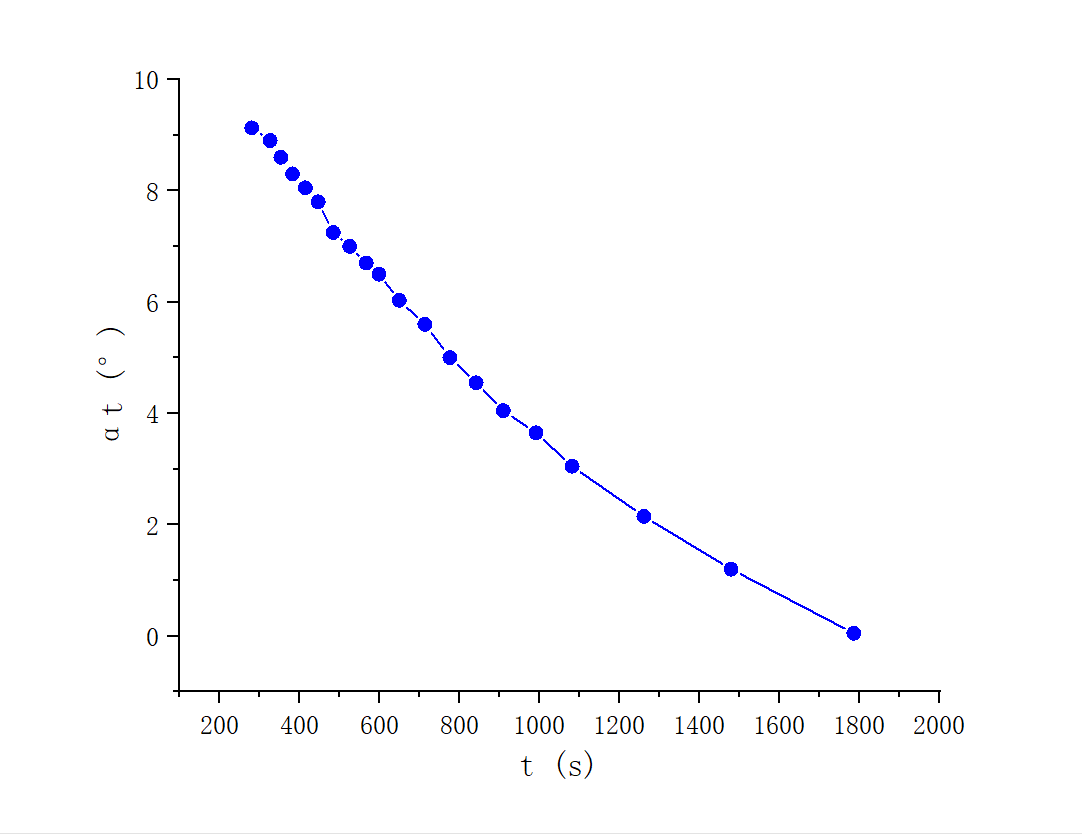
\includegraphics[width=0.90\textwidth]{2.png}
				\bicaption{添加盐酸浓度为$3.13\ \ {\rm M}$下混合液$t-\alpha_{t}$图像}{The mixed solution $t-\alpha_{t}$ image with $3.13\ \ {\rm M}$ added hydrochloric acid}
			\end{figure}
			\par
			\textbf{图3}展示了盐酸浓度为$4.12\ \ {\rm M}$时,蔗糖转化反应的旋光度随时间t的变化。做出相应的$t-\alpha_{t}$图像如\textbf{图3}所示:\par
			\begin{table}[!h]
				\arrayrulecolor{Maroon}
				\centering
				\zihao{5}
				\bicaption{添加盐酸浓度为$4.12\ \ {\rm M}$下混合液$t-\alpha_{t}$测量数据}{The measurement data of the mixed solution with $4.12\ \ {\rm M}$ added hydrochloric acid}
				\begin{tabular}{ccccccccc}
					\toprule
					编号 & $t/{\rm s}$ & $\alpha^{\prime}_{t}/^{\circ}$ & $\alpha_{t}/^{\circ}$&&编号& $t/{\rm s}$ & $\alpha^{\prime}_{t}/^{\circ}$ & $\alpha_{t}/^{\circ}$\\
					\midrule
					1 & 157 & 9.40 & 9.43 &  & 10 & 642  & 2.90  & 2.93  \\
					2 & 184 & 8.85 & 8.88 &  & 11 & 708  & 2.40  & 2.43  \\
					3 & 221 & 8.10 & 8.13 &  & 12 & 760  & 1.95  & 1.98  \\
					4 & 268 & 7.60 & 7.63 &  & 13 & 823  & 1.60  & 1.63  \\
					5 & 306 & 6.50 & 6.53 &  & 14 & 882  & 1.20  & 1.23  \\
					6 & 340 & 5.85 & 5.88 &  & 15 & 934  & 0.80  & 0.83  \\
					7 & 391 & 5.05 & 5.08 &  & 16 & 1024 & 0.35  & 0.38  \\
					8 & 458 & 4.20 & 4.23 &  & 17 & 1086 & -0.05 & -0.02 \\
					9 & 520 & 3.55 & 3.58 &  &    &      &       &       \\
					\bottomrule
				\end{tabular}
			\end{table}
			\begin{figure}[!h]
				\centering
				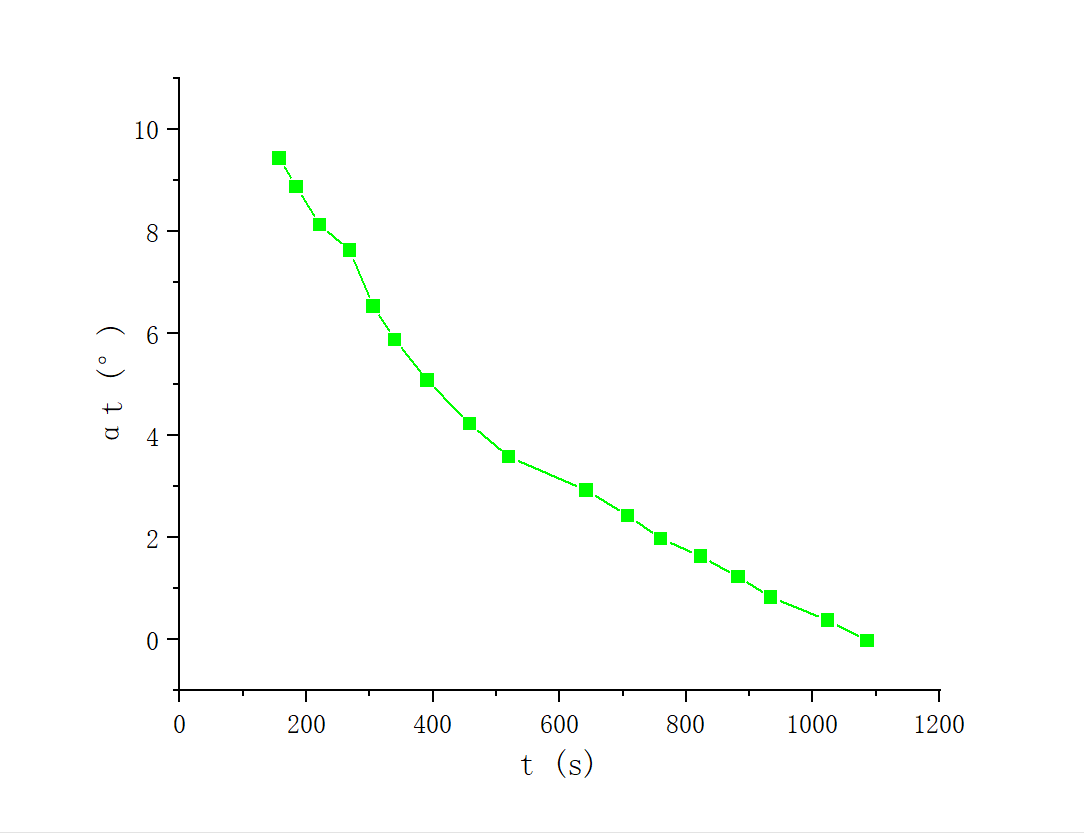
\includegraphics[width=0.90\textwidth]{3.png}
				\bicaption{添加盐酸浓度为$4.12\ \ {\rm M}$下混合液$t-\alpha_{t}$图像}{The mixed solution $t-\alpha_{t}$ image with $4.12\ \ {\rm M}$ added hydrochloric acid}
			\end{figure}
			\par
			\textbf{图4}展示了盐酸浓度为$6.16\ \ {\rm M}$时,蔗糖转化反应的旋光度随时间t的变化。$6.16\ \ {\rm M}$时反应时间较短,变为左旋之前的数据点相对较少,因此测量了一部分左旋后的数据,笔者认为其引入的误差较小,详细见误差分析部分。\par
			\begin{table}[!h]
				\arrayrulecolor{Maroon}
				\centering
				\zihao{5}
				\bicaption{添加盐酸浓度为$6.16\ \ {\rm M}$下混合液$t-\alpha_{t}$测量数据}{The measurement data of the mixed solution with $6.16\ \ {\rm M}$ added hydrochloric acid}
				\begin{tabular}{ccccccccc}
					\toprule
					编号 & $t/{\rm s}$ & $\alpha^{\prime}_{t}/^{\circ}$ & $\alpha_{t}/^{\circ}$&&编号& $t/{\rm s}$ & $\alpha^{\prime}_{t}/^{\circ}$ & $\alpha_{t}/^{\circ}$\\
					\midrule
					1 & 155 & 6.75 & 6.78 &  & 7  & 332 & 1.75  & 1.78  \\
					2 & 176 & 5.05 & 5.08 &  & 8  & 361 & 1.15  & 1.18  \\
					3 & 200 & 4.55 & 4.58 &  & 9  & 388 & 0.90  & 0.93  \\
					4 & 248 & 3.20 & 3.23 &  & 10 & 422 & 0.20  & 0.23  \\
					5 & 280 & 2.80 & 2.83 &  & 11 & 448 & -0.05 & -0.02 \\
					6 & 303 & 2.10 & 2.13 &  & 12 & 476 & -0.40 & -0.37 \\
					\bottomrule
				\end{tabular}
			\end{table}
			做出相应的$t-\alpha_{t}$图像如\textbf{图4}所示:
			\begin{figure}[!h]
				\centering
				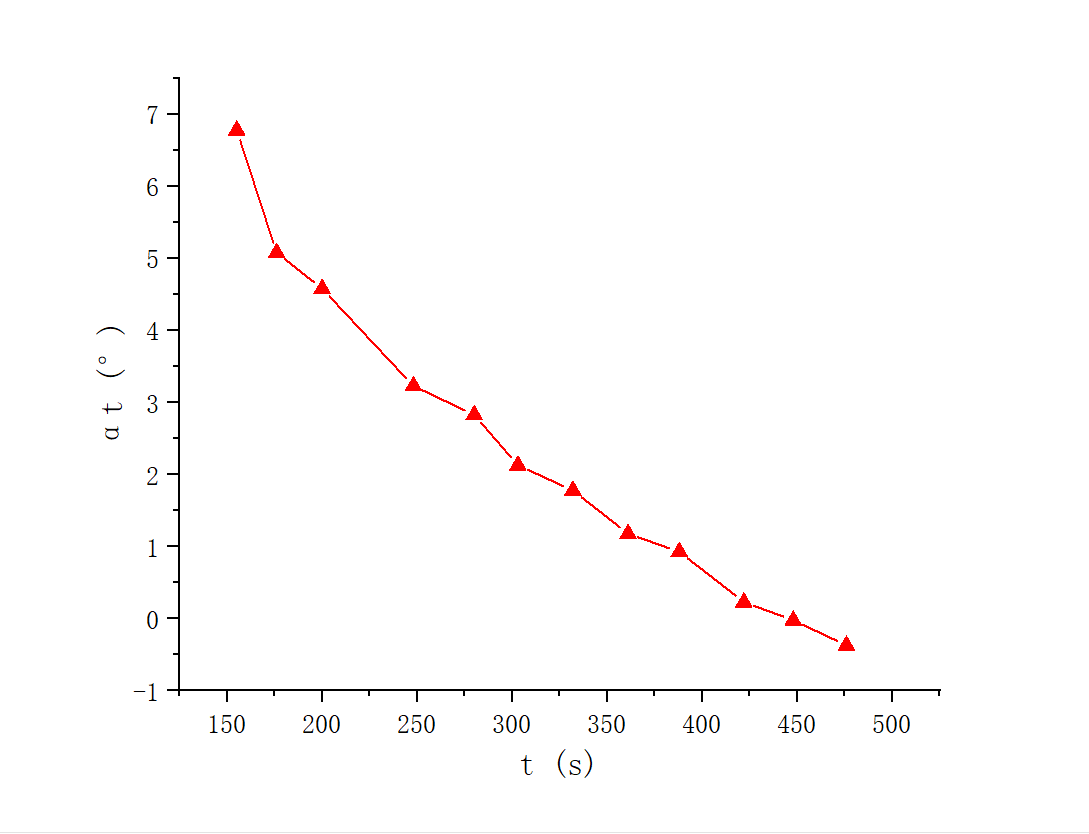
\includegraphics[width=0.90\textwidth]{4.png}
				\bicaption{添加盐酸浓度为$6.16\ \ {\rm M}$下混合液$t-\alpha_{t}$图像}{The mixed solution $t-\alpha_{t}$ image with $6.16\ \ {\rm M}$ added hydrochloric acid}
			\end{figure}
			\par
			可以注意到,\textbf{图2}、\textbf{图3}、\textbf{图4}中吸光度的变化趋势是相似的,但是在吸光度的变化速率上有所不同,盐酸浓度越高,吸光度的变化速率越大。这一对比在\textbf{图5}中示出:\par
			\begin{figure}[!h]
				\centering
				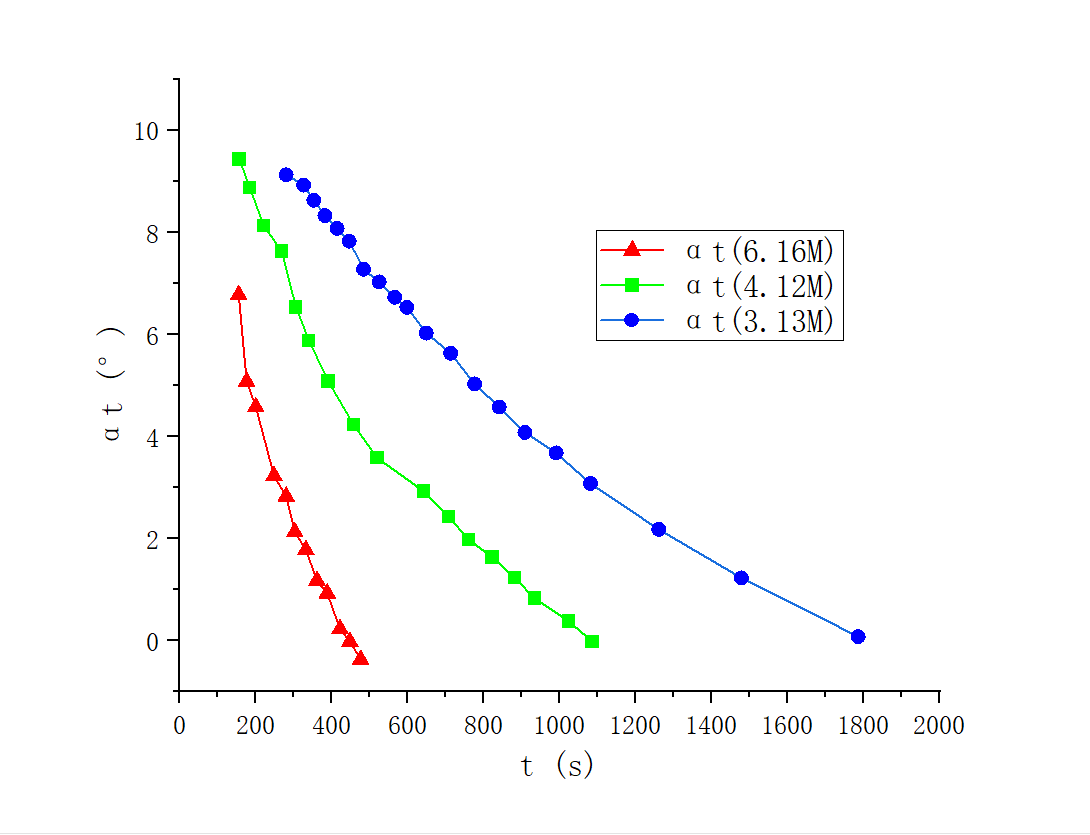
\includegraphics[width=0.90\textwidth]{5.png}
				\bicaption{不同盐酸浓度下混合液$\alpha_{t}-t$图}{$\alpha_{t}-t$ diagram under different hydrochloric acid concentration}
			\end{figure}
			\par

			\subsubsection{$\alpha_{\infty}$的测定}
			测量保留备用的第1次测定时$6.16\ \ {\rm M}$盐酸溶液与蔗糖溶液的混合液的旋光度,重复测量3次,读取旋光仪的原始旋光角$\alpha^{\prime}_{\infty}$,根据
			$$
			\alpha_{\infty}=\alpha^{\prime}_{\infty}-\alpha
			$$
			\begin{table}[!h]
				\centering
				\zihao{5}
				\bicaption{$\alpha_{\infty}$测量数据}{$\alpha_{\infty}$ measurement data}
				\begin{tabular}{cccc}
					\toprule
					编号 & 1 & 2 & 3 \\
					\midrule
					$\alpha^{\prime}_{\infty} / ^{\circ}$ & -4.05 & -4.10 & -4.05 \\
							$\alpha_{\infty} / ^{\circ}$ & -4.02 & -4.07 & -4.02 \\
					\bottomrule
				\end{tabular}
			\end{table}
			\par
			根据\textbf{表5}数据,计算$\alpha_{\infty}$的平均值为:
			$$
			\alpha_{\infty}=-4.04^{\circ}
			$$\par
			因此$\alpha_{\infty}$的标准偏差为:
			$$
			\sigma_{\alpha_{\infty}}=\sqrt{\frac{0.02^{2}+0.02^{2}+0.03^{2}}{3-1}}=0.02^{\circ}
			$$\par
			故$\alpha_{\infty}$为:
			$$
			\alpha_{\infty}=(-4.04\pm 0.02)^{\circ}
			$$\par


		\subsection{数据处理结果与分析}
			\subsubsection{蔗糖转化反应关于蔗糖的反应级数}
			根据\textbf{表2}、\textbf{表3}和\textbf{表4}的数据以及$\alpha_{\infty}=-4.04^{\circ}$,计算不同盐酸浓度下的$(\alpha_{t}-\alpha_{\infty})$和${\rm ln}(\alpha_{t}-\alpha_{\infty})$数据,各项数据示于\textbf{表6}。\par
			\begin{table}[!h]
				\centering
				\zihao{5}
				\bicaption{不同盐酸浓度下混合液$(\alpha_{t}-\alpha_{\infty})$和${\rm ln}(\alpha_{t}-\alpha_{\infty})$数据}{Data of $(\alpha_{t}-\alpha_{\infty})$和${\rm ln}(\alpha_{t}-\alpha_{\infty})$ under different hydrochloric acid concentration}
				\begin{tabular}{ccccccccc}
					\toprule
					\multicolumn{9}{c}{3.13M}																							   \\
					序号 & $t/{\rm s}$ & $\alpha_{t}-\alpha_{\infty}/ ^{\circ}$ & ${\rm ln}(\alpha_{t}-\alpha_{\infty})$ &  & 序号 & $t/{\rm s}$ & $\alpha_{t}-\alpha_{\infty}/ ^{\circ}$ & ${\rm ln}(\alpha_{t}-\alpha_{\infty})$ \\
					\midrule
					1  & 280           & 13.17               & 2.578   &  & 11 & 649           & 10.07               & 2.310   \\
					2  & 326           & 12.97               & 2.563   &  & 12 & 713           & 9.67                & 2.269   \\
					3  & 353           & 12.67               & 2.539   &  & 13 & 776           & 9.07                & 2.205   \\
					4  & 382           & 12.37               & 2.515   &  & 14 & 841           & 8.62                & 2.154   \\
					5  & 414           & 12.12               & 2.495   &  & 15 & 909           & 8.12                & 2.094   \\
					6  & 446           & 11.87               & 2.474   &  & 16 & 991           & 7.72                & 2.044   \\
					7  & 484           & 11.32               & 2.427   &  & 17 & 1081          & 7.12                & 1.963   \\
					8  & 525           & 11.07               & 2.404   &  & 18 & 1261          & 6.22                & 1.828   \\
					9  & 566           & 10.77               & 2.377   &  & 19 & 1479          & 5.27                & 1.662   \\
					10 & 598           & 10.57               & 2.358   &  & 20 & 1786          & 4.12                & 1.416   \\
					\midrule
					\multicolumn{9}{c}{4.12M}                                                                                              \\
					序号 & $t/{\rm s}$ & $\alpha_{t}-\alpha_{\infty}/ ^{\circ}$ & ${\rm ln}(\alpha_{t}-\alpha_{\infty})$ &  & 序号 & $t/{\rm s}$ & $\alpha_{t}-\alpha_{\infty/ ^{\circ}}$ & ${\rm ln}(\alpha_{t}-\alpha_{\infty})$ \\
					\midrule
					1  & 157           & 13.47               & 2.600   &  & 10 & 642           & 6.97                & 1.942   \\
					2  & 184           & 12.92               & 2.559   &  & 11 & 708           & 6.47                & 1.867   \\
					3  & 221           & 12.17               & 2.499   &  & 12 & 760           & 6.02                & 1.795   \\
					4  & 268           & 11.67               & 2.457   &  & 13 & 823           & 5.67                & 1.735   \\
					5  & 306           & 10.57               & 2.358   &  & 14 & 882           & 5.27                & 1.662   \\
					6  & 340           & 9.92                & 2.295   &  & 15 & 934           & 4.87                & 1.583   \\
					7  & 391           & 9.12                & 2.210   &  & 16 & 1024          & 4.42                & 1.486   \\
					8  & 458           & 8.27                & 2.113   &  & 17 & 1086          & 4.02                & 1.391   \\
					9  & 520           & 7.62                & 2.031   &  &    &               &                     &               \\
					\midrule
					\multicolumn{9}{c}{6.16M}                                                                                             \\
					\midrule
					序号 & $t/{\rm s}$ & $\alpha_{t}-\alpha_{\infty}/ ^{\circ}$ & ${\rm ln}(\alpha_{t}-\alpha_{\infty})$ &  & 序号 & $t/{\rm s}$ & $\alpha_{t}-\alpha_{\infty}/ ^{\circ}$ & ${\rm ln}(\alpha_{t}-\alpha_{\infty})$ \\
					\midrule
					1  & 155           & 10.82               & 2.381   &  & 10 & 332           & 5.82                & 1.761   \\
					2  & 176           & 9.12                & 2.210   &  & 11 & 361           & 5.22                & 1.652   \\
					3  & 200           & 8.62                & 2.154   &  & 12 & 388           & 4.97                & 1.603    \\
					4  & 248           & 7.27                & 1.984   &  & 13 & 422           & 4.27                & 1.451   \\
					5  & 280           & 6.87                & 1.927   &  & 14 & 448           & 4.02                & 1.391   \\
					6  & 303           & 6.17                & 1.820   &  & 15 & 476           & 3.67                & 1.300   \\
					\bottomrule
					\end{tabular}
					\end{table}
					根据\textbf{表6}数据,作出不同盐酸浓度下混合液${\rm ln}(\alpha_{t}-\alpha_{\infty})-t$散点图,并用origin进行线性拟合,作出不同盐酸浓度下混合液${\rm ln}(\alpha_{t}-\alpha_{\infty})-t$拟合直线,如\textbf{图6}所示:\par
					\vbox{}
					\vbox{}
					\begin{figure}[!h]
						\centering
						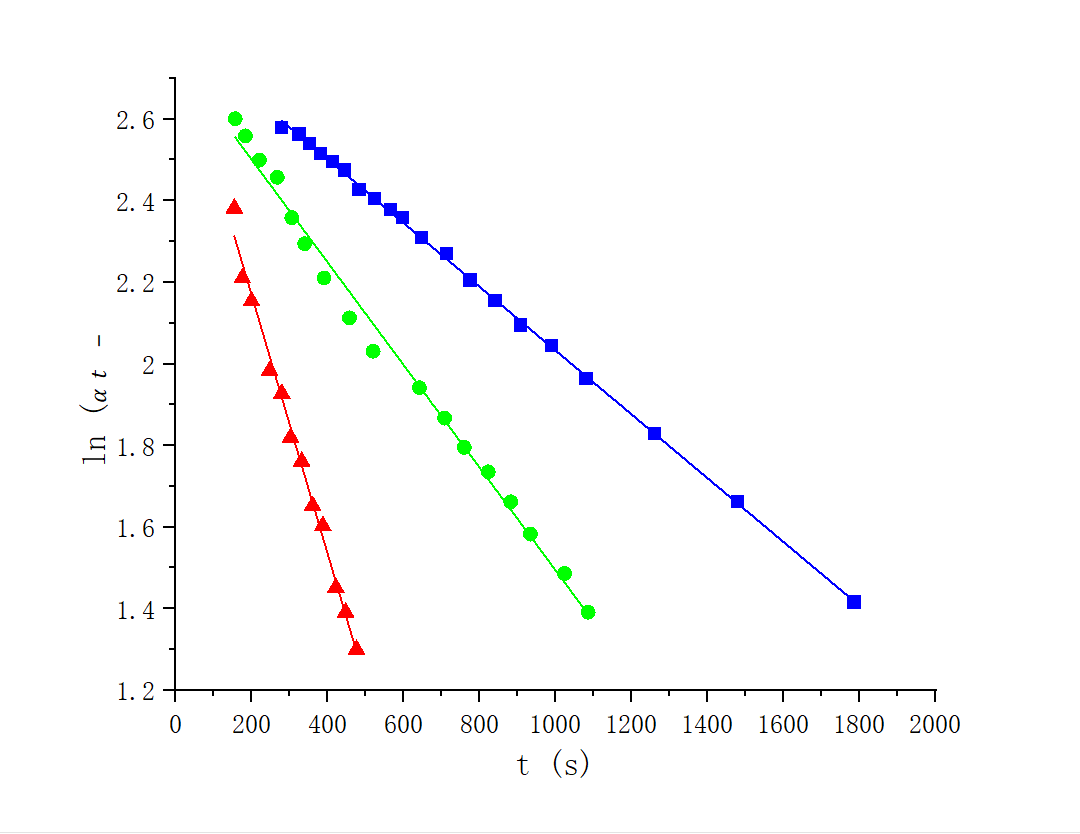
\includegraphics[width=0.70\textwidth]{6.png}
						\bicaption{不同光源下$\rm (A3)$溶液的吸收光谱}{Absorption spectrum of (A) solution under different light sources}
					\end{figure}
					根据\textbf{图6}可以看出,不同盐酸浓度下${\rm ln}(\alpha_{t}-\alpha_{\infty})-t$都具有良好的线性关系,进一步的可以计算出$3.13\ \ {\rm M}$、$4.12\ \ {\rm M}$、$6.16\ \ {\rm M}$盐酸浓度下的回归直线方程分别为:
					$$
					{\rm ln}(\alpha_{t}-\alpha_{\infty})=-7.82\times10^{-4}t/s+2.815,\ \ R=-0.9998
					$$
					$$
					{\rm ln}(\alpha_{t}-\alpha_{\infty})=-1.26\times10^{-3}t/s+2.752,\ \ R=-0.9960
					$$
					$$
					{\rm ln}(\alpha_{t}-\alpha_{\infty})=-3.17\times10^{-3}t/s+2.803,\ \ R=-0.9963
					$$
					根据一级反应的动力学特征:
					$$
					{\rm ln}\frac{c_{0}}{c_{t}}=kt
					$$
					可以判断$\rm H^{+}$浓度固定的条件下,蔗糖转化反应为一级反应。
					\subsubsection{反应速率常数$k$和半衰期$t_{1/2}$}
					根据
					$$
					{\rm ln}(\alpha_{t}-\alpha_{\infty})=kt+{\rm ln}(\alpha_{0}-\alpha_{\infty})
					$$
					可以用拟合直线的斜率$a$计算速率常数$k$,即:
					$$
					k=-a
					$$
					又因为一级反应的半衰期满足:
					$$
					t_{1/2}=\frac{0.693}{k}
					$$
					由\textbf{3.2.1}中数据可得:
					$$\left\{\begin{aligned}
					k_{3.13M}&=7.82\times10^{-4}\ \ {\rm s^{-1}}\\
					k_{4.12M}&=1.26\times10^{-3}\ \ {\rm s^{-1}}\\
					k_{6.16M}&=3.17\times10^{-3}\ \ {\rm s^{-1}}
					\end{aligned}\right.$$
					$$\left\{\begin{aligned}
					t_{1/2,3.13M}&=887.5\ \ {\rm s}\\
					t_{1/2,4.12M}&=550.8\ \ {\rm s}\\
					t_{1/2,6.16M}&=218.6\ \ {\rm s}
						\end{aligned}\right.$$
					\par

					\subsubsection{蔗糖转化反应关于$\rm H^{+}$的反应级数}
					考虑H$^{+}$对反应速率的影响,有
					$$
					k=k_{0}+k_{\rm H^{+}}c^{n}_{\rm H^{+}}
					$$
					其中$k_{0}$是$c_{\rm H^{+}}\rightarrow0$时的反应速率常数,$k_{\rm H^{+}}$为酸催化速率常数,$k$为表观速率常数,$n$为$\rm H^{+}$的反应级数。两边取以$e$为底的对数,即得
					$$
					{\rm ln}(k-k_{0})=n{\rm ln}c_{\rm H^{+}}+{\rm ln}k_{\rm H^{+}}
					$$
					故作出${\rm ln}(k-k_{0})-{\rm ln}c_{\rm H^{+}}$拟合直线,由直线斜率即可求出$\rm H^{+}$的反应级数$n$。\par 
					因为蔗糖在非质子溶剂中是稳定的,因此可以认为当$c_{\rm H^{+}}$浓度为0时,反应无法发生,即$k_{0}=0$,根据$k_{0}$和\textbf{3.2.2}中数据,计算$c_{\rm H^{+}}=\frac{1}{2}c({\rm HCl})$,${\rm ln}c_{\rm H^{+}}$与${\rm ln}(k-k_{0})$,计算结果示于\textbf{表7}。做出${\rm ln}c_{\rm H^{+}}-{\rm ln}(k-k_{0})$散点图,并用origen进行线性拟合,作出${\rm ln}c_{\rm H^{+}}-{\rm ln}(k-k_{0})$拟合直线,如\textbf{图7}所示。
					\begin{table}[h]
						\centering
						\zihao{5}
						\bicaption{$c_{\rm H^{+}}$,${\rm ln}c_{\rm H^{+}}$与${\rm ln}(k-k_{0})$计算结果}{Calculation results of $c_{\rm H^{+}}$, ${\rm ln}c_{\rm H^{+}}$ and ${\rm ln}(k-k_{0})$ }
						\begin{tabular}{cccc}
							\toprule
							
							$c_{\rm H^{+}} / {\rm M}$ & ${\rm ln}c_{\rm H^{+}}$ & $(k-k_{0})/{\rm 10^{-4} \ \ s^{-1}}$ & ${\rm ln}(k-k_{0})$\\
							\midrule
							1.565 & 0.4479 &  7.82 &  2.057\\
							2.060 & 0.7227 & 12.6 & 2.534 \\
							3.080 & 1.125 & 31.7 & 3.456 \\
							\bottomrule
						\end{tabular}
					\end{table}
					\par
					\begin{figure}[h]
						\centering
						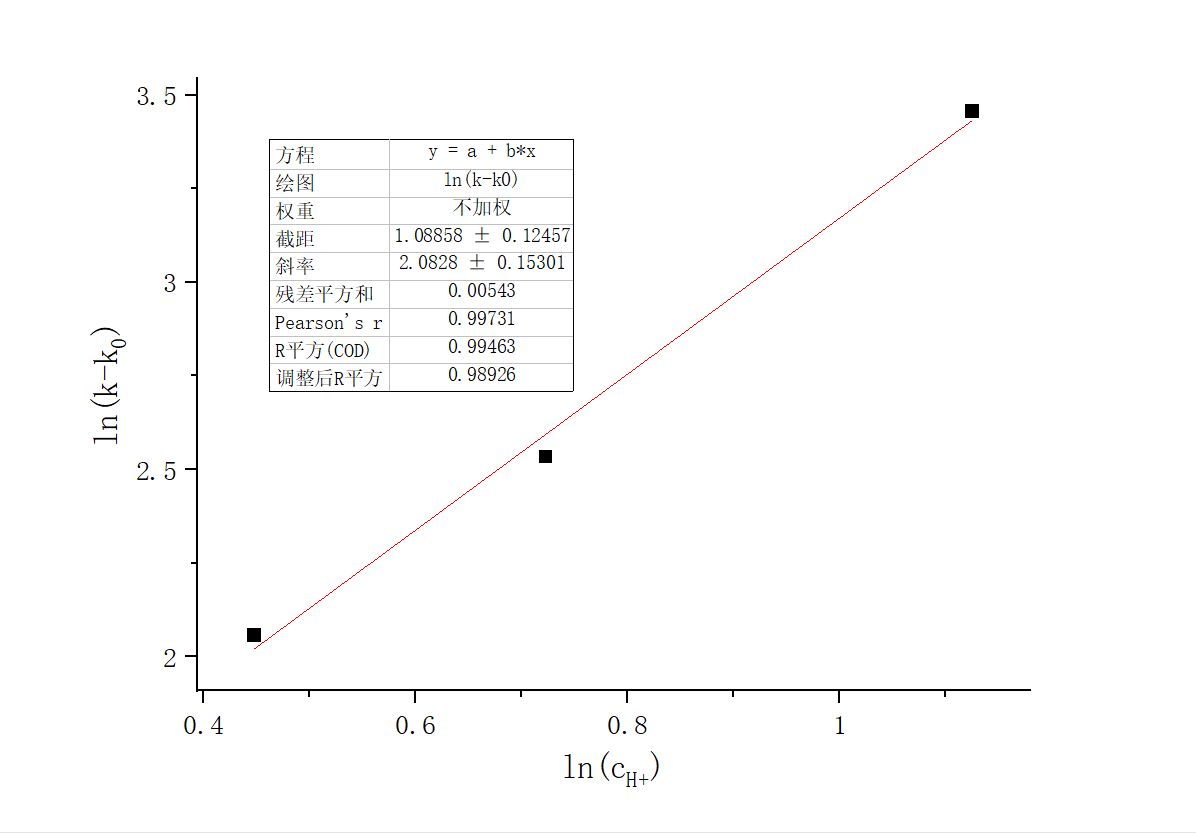
\includegraphics[width=0.70\textwidth]{7.png}
						\bicaption{${\rm ln}c_{\rm H^{+}}-{\rm ln}(k-k_{0})$拟合直线}{${\rm ln}c_{\rm H^{+}}-{\rm ln}(k-k_{0})$ fitting straight line}
					\end{figure}
					\par
					根据\textbf{图7}可以看出,${\rm ln}c_{\rm H^{+}}-{\rm ln}(k-k_{0})$具有良好的线性关系,其回归方程为:
					$$
					{\rm ln}(k-k_{0})=2.0828\ \ {\rm ln}c_{\rm H^{+}}+1.08858,\ \ R=0.9971
					$$
					故$\rm H^{+}$的反应级数
					$$
					n=2.0828\approx2
					$$
					即对氢离子为二级反应。

					\section{讨论与结论}
					\subsection{实验讨论}
					\subsubsection{测量左旋数据的影响}
					在测量$6.16\ \ {\rm M}$盐酸溶液与蔗糖溶液的混合液的旋光度时,由于反应速率较快,变为左旋之前的数据点相对较少,因此测量了一部分左旋后的数据。笔者认为其引入的误差较小,因为最终计算和拟合是基于$(\alpha_{t}-\alpha_{\infty})$的,这与测量出的旋光度为正值或者负值无关,因此测量左旋数据的不会对最终结果产生系统性误差。但因为其他组的实验数据中没有测量左旋数据,因此可能此数据与其他组的数据无法进行较好的横向对比,但是笔者认为这不会对最终结果造成很大的影响。
					\subsubsection{误差来源分析}
					笔者认为本次实验中误差主要来源于以下几个方面:
					\begin{enumerate}
						\item \textbf{人眼的精确度不够}:在实际测量过程中,需要手动调节旋光仪度盘调节手轮至三分视场消失、视野暗度相同,但每一次人眼判断暗视场出现的位置会有所不同,比如笔者眼神不太好,这导致在他看来‘三分视场消失、视野暗度相同’是一个很大的区间,这必然会引入较大的误差。\par
						\item \textbf{体系未充分混合,旋光管未充分润洗}:在实验过程中,蔗糖溶液一半倒入盐酸后就会开始计时。在倒完蔗糖后,实验人员需要完成,摇匀、润洗旋光管、转移混合液等操作。这些操作都需要一定的时间,但本实验又要求尽快开始测量,这必然会导致操作的匆忙,很多步骤如润洗、混合无法充分进行,这也是误差的来源之一。\par
					\end{enumerate}
					\subsubsection{实验的改进}
					笔者认为本实验可以改进的地方有:
					\begin{enumerate}
						\item \textbf{降低盐酸浓度}:本实验中盐酸浓度较高,导致反应速率较快,这使得实验人员在操作时很容易出现匆忙的情况,这也是误差的来源之一。因此可以考虑降低盐酸浓度,使得反应速率降低,这样可以给实验人员更多的操作时间,从而减少误差,以本实验为例,从\textbf{图6}可以明显看出,$3.13\ \ {\rm M}$盐酸组的线性度要好于其他两组。但这样必然会造成实验时间的延长,因此需要在实验时间和误差之间做出权衡。\par
						\item \textbf{使用更加数字化的测量方式}:这仅仅是一个猜想,比如可以将使用光强探测器将三分视野的亮度数值化,这样实验人员仅需比较数值差异就可以读取旋光度,可以减少人眼的误差(虽然感觉这样就变成电子旋光仪了)。\par
					\end{enumerate}
				\subsection{实验结论}
				本实验利用目视旋光仪测定蔗糖转化过程中体系旋光度的变化,间接得到了蔗糖的浓度变化,从而计算蔗糖转化反应的化学反应动力学常数。实验中加入浓度为$3.13\ \ {\rm M}$、$4.12\ \ {\rm M}$和$6.16\ \ {\rm M}$的盐酸时,蔗糖转化反应的速率常数$k$分别为$7.82\times10^{-4}\ \ s^{-1}$、$1.26\times10^{-3}\ \ s^{-1}$和$3.17\times10^{-3}\ \ s^{-1}$。计算了对应的半衰期$t_{1/2}$分别为$885\ \ s$、$550\ \ s$和$220\ \ s$。实验结果验证了蔗糖转化反应的对于蔗糖为一级反应,对氢离子为二级反应。


					



	\vbox{}
	\section{Supporting Information}
		本实验所有的原始数据、python代码、实验报告的 LaTeX 源代码均可在\par
		 $\rm{https://github.com/wzhstat/Physical\_Chemistry\_Experiments}$找到,原始数据也会邮箱发送给实验老师。
\vbox{}  
%参考文献
\bibliographystyle{unsrt}
\bibliography{cite}
\end{document}